%%
%% Copyright 2025 Oxford University Press
%%
%% This file is part of the 'oup-authoring-template Bundle'.
%% ---------------------------------------------
%%
%% It may be distributed under the conditions of the LaTeX Project Public
%% License, either version 1.3 of this license or (at your option) any
%% later version.  The latest version of this license is in
%%    https://www.latex-project.org/lppl.txt
%% and version 1.2 or later is part of all distributions of LaTeX
%% version 1999/12/01 or later.
%%
%% The list of all files belonging to the 'oup-authoring-template Bundle' is
%% given in the file `manifest.txt'.
%%

%%%CONTEMPORARY%%%
\documentclass[unnumsec,webpdf,contemporary,large]{oup-authoring-template}%

\graphicspath{{Fig/}}

\begin{document}

\journaltitle{Bioinformatics}
\DOI{DOI added during production}
\copyrightyear{2026}
\pubyear{2026}
\vol{XX}
\issue{X}
\access{Advance Access Publication Date: to be assigned}
\appnotes{Original Article}

\firstpage{1}

\title[KGAMA for molecular property prediction]{KGAMA: knowledge-enhanced graph-anchor multimodal alignment for molecular property prediction}

\author[1,$\ast$]{Yunyun Niu}
\author[1]{Shuaiyao Fan}

\address[1]{\orgdiv{School of Artificial Intelligence}, \orgname{China University of Geosciences (Beijing)}, \orgaddress{\city{Beijing}, \country{China}}}

\corresp[$\ast$]{Corresponding author. \href{mailto:your-email@example.com}{your-email@example.com}}

\abstract{
\textbf{Motivation:} Multimodal molecular learning is attractive for property prediction because graphs, SMILES, fingerprints and text provide complementary information. In practice, however, public molecular text is often noisy and loosely constrained, whereas exhaustive multimodal alignment can introduce instability during training.\\
\textbf{Results:} We propose KGAMA, a knowledge-enhanced graph-anchor multimodal alignment framework for molecular property prediction. KGAMA combines four modalities---molecular graphs, SMILES sequences, molecular fingerprints and rewritten scientific text---within a pretraining--finetuning pipeline. We first construct a knowledge-enhanced text pipeline that rewrites PubChem descriptions with a large language model and injects 11 RDKit-derived physicochemical descriptors. We then perform graph-centered contrastive pretraining, treating the molecular graph as the semantic anchor and using uncertainty-aware adaptive weighting to stabilize cross-modal optimization. During finetuning, modality-specific features are integrated by cross-attention for downstream prediction. On 9 MoleculeNet benchmarks, KGAMA achieves the best overall performance among competitive baselines, with AUROC values of 0.872 on BACE, 0.930 on BBBP, 0.939 on ClinTox, 0.841 on Tox21, 0.712 on ToxCast and 0.669 on SIDER, and RMSE values of 0.831 on ESOL, 1.512 on FreeSolv and 0.655 on Lipophilicity. Ablation and visualization analyses support the contribution of knowledge-enhanced text, graph-centered alignment and adaptive multimodal fusion.\\
\textbf{Availability and implementation:} Code and processed data will be made available at a public repository upon acceptance.\\
\textbf{Contact:} \href{mailto:your-email@example.com}{your-email@example.com}\\
\textbf{Supplementary information:} Supplementary data are available online.
}

\keywords{molecular property prediction, multimodal learning, graph representation learning, contrastive learning, drug discovery}

\maketitle

\section{Introduction}
Molecular property prediction is a central task in computational drug discovery because it supports early-stage prioritization of candidate compounds with favorable absorption, distribution, metabolism, excretion and toxicity profiles. Recent progress in deep learning has substantially improved molecular representation learning, enabling predictive models to extract useful signals from graph topology, substructure composition and sequence-based encodings. Even so, the biochemical behaviour of a molecule is governed by heterogeneous structural and pharmacological factors, and no single modality is sufficient to characterize the full spectrum of evidence relevant to downstream prediction.

Multimodal learning provides a natural route to address this limitation. Molecular graphs encode topological connectivity, SMILES strings preserve a linearized chemical syntax, fingerprints summarize substructure occurrence patterns, and text descriptions can expose pharmacological or physicochemical knowledge that is not explicit in structural encodings alone. Prior studies have shown that combining multiple molecular modalities can improve property prediction. Nevertheless, two practical bottlenecks remain. First, public molecular text is often noisy, verbose and weakly constrained by quantitative chemical evidence, which reduces the utility of text representations. Second, full pairwise alignment across multiple modalities may amplify noise and make optimization unstable, especially when the modalities differ substantially in information content and uncertainty.

To address these issues, we propose KGAMA, a knowledge-enhanced graph-anchor multimodal alignment framework for molecular property prediction. KGAMA is built around two ideas. The first is knowledge-enhanced text rewriting, in which raw molecular descriptions are cleaned and rewritten with the help of a large language model and explicit RDKit-derived physicochemical descriptors. The second is graph-centered multimodal alignment, in which the molecular graph is treated as the semantic anchor and auxiliary modalities are aligned to this anchor through contrastive pretraining with uncertainty-aware dynamic weighting. The resulting multimodal representations are then fused by cross-attention for downstream task prediction.

This study makes three main contributions. First, we develop a practical knowledge enhancement pipeline that improves the density, consistency and task relevance of molecular text. Second, we introduce a graph-centered alignment strategy that avoids redundant auxiliary-to-auxiliary matching and improves the robustness of multimodal representation learning. Third, we perform systematic evaluation on 9 MoleculeNet benchmarks spanning both classification and regression tasks, where KGAMA shows strong and consistent gains over representative graph, self-supervised and multimodal baselines.

\section{Materials and Methods}
\subsection{Overview of KGAMA}
KGAMA is a multimodal molecular property prediction framework that combines four complementary views of each molecule: graph, sequence, fingerprint and text. The framework follows a pretraining--finetuning paradigm. In the pretraining stage, modality-specific encoders project each molecular view into a shared latent space, where graph-centered contrastive learning is used to align the auxiliary modalities with the molecular graph. In the finetuning stage, the pretrained encoders are transferred to downstream prediction tasks and their representations are fused by cross-attention and a multilayer perceptron predictor.

The model contains three major components: modality-specific encoders, representation mapping layers and a fusion-prediction module. The modality-specific encoders produce graph, sequence, fingerprint and text representations, denoted by $F_g$, $F_s$, $F_f$ and $F_t$, respectively. Mapping layers project these modality-specific features into a common representation space. The fusion-prediction module then models cross-modal interaction and generates the final property prediction. The overall workflow of KGAMA is illustrated in Figure~\ref{fig:framework}.

\begin{figure*}[t]
    \centering
    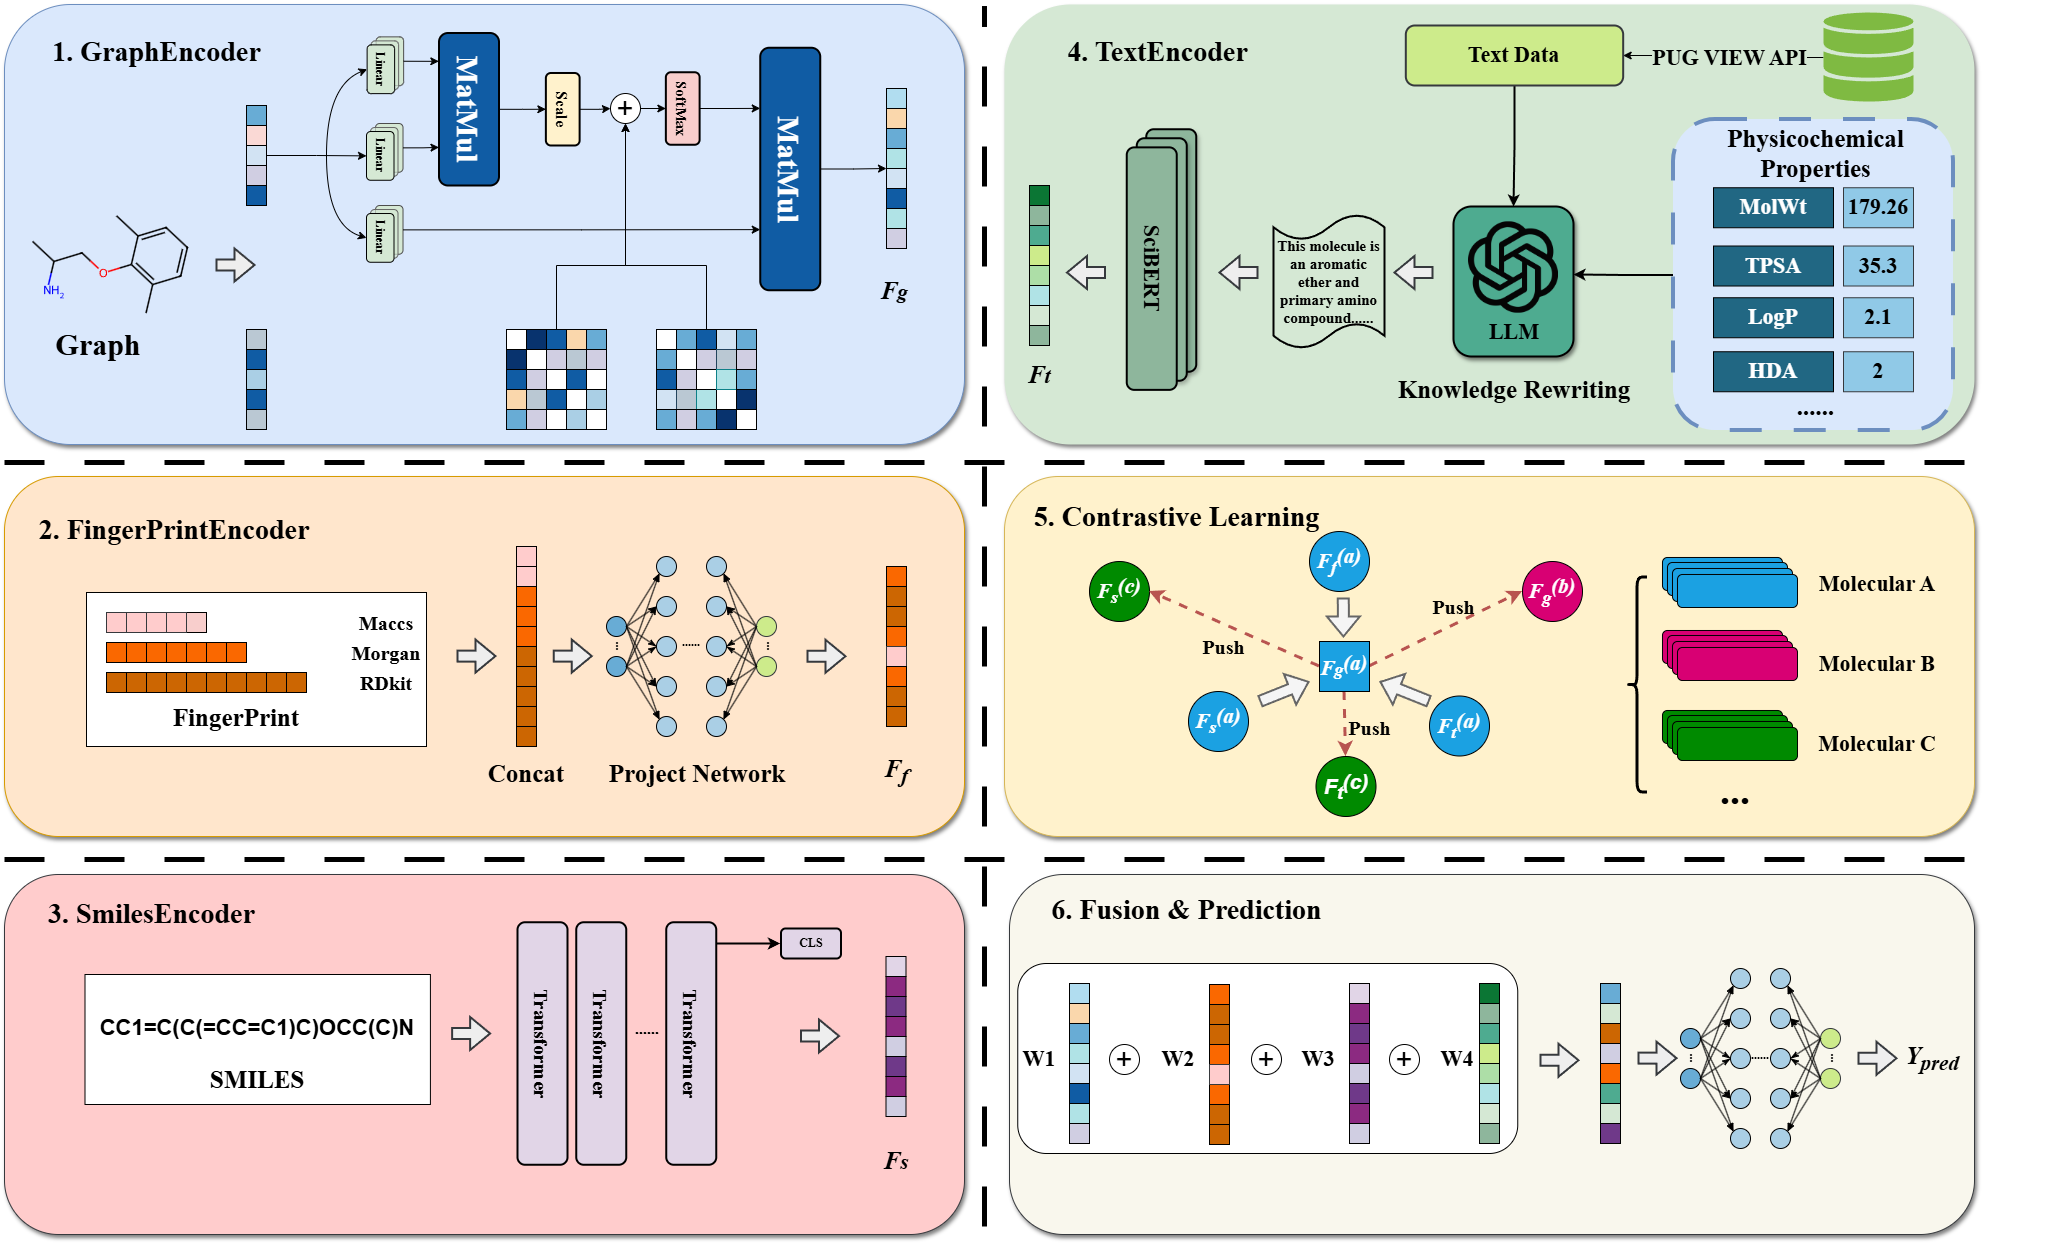
\includegraphics[width=\textwidth]{figures/fig1_framework.png}
    \caption{Overall framework of KGAMA. The model integrates graph, SMILES, fingerprint and knowledge-enhanced text modalities within a graph-centered pretraining and downstream fusion pipeline.}
    \label{fig:framework}
\end{figure*}

\subsection{Graph encoder as semantic anchor}
The molecular graph is treated as the semantic anchor of KGAMA because it provides the most direct and stable representation of molecular structure. We use Graphormer as the graph encoder. In contrast to conventional message passing architectures with limited receptive fields, Graphormer captures long-range structural dependencies through a combination of centrality encoding, spatial encoding and edge encoding. This design allows the model to jointly encode atom importance, shortest-path information and bond-type information, yielding a graph representation with high structural fidelity.

Using the graph branch as the anchor serves two purposes. First, it grounds the multimodal representation in chemically faithful topology. Second, it reduces the combinatorial burden of pairwise multimodal alignment by aligning each auxiliary modality only to the graph representation rather than to every other modality.

\subsection{Sequence, fingerprint and text encoders}
The sequence branch models SMILES strings as linearized molecular expressions and captures long-range symbolic dependencies that may be overlooked by purely graph-based representations. The fingerprint branch encodes substructure statistics and is particularly useful for properties associated with characteristic functional groups or fragment counts. In practice, fingerprint features complement graph representations by providing a compact summary of global composition patterns.

The text branch provides semantic information about molecular properties and biological effects. To improve its reliability, KGAMA adopts a knowledge-enhanced rewriting pipeline. For each molecule, we first retrieve raw textual descriptions from PubChem and compute 11 physicochemical descriptors with RDKit, including features such as LogP and topological polar surface area. A large language model is then used to rewrite the original description under three constraints: domain-expert role conditioning, joint use of raw text and quantitative descriptors, and explicit suppression of irrelevant content such as patent identifiers, historical anecdotes and commercial names. The rewritten text is subsequently encoded with SciBERT, yielding dense task-relevant semantic representations.

\subsection{Pretraining data construction}
We constructed a multimodal pretraining dataset from PubChem. Approximately 300,000 small-molecule SMILES strings were initially sampled. All molecules were standardized with RDKit, and invalid, duplicate or malformed structures were removed. Molecules overlapping with downstream benchmark datasets were also excluded using unique identifiers. After filtering, approximately 220,000 distinct molecules were retained.

For each retained molecule, raw text descriptions were retrieved through the PubChem API and processed by the knowledge enhancement pipeline described above. In parallel, two-dimensional molecular graphs, SMILES sequences and fingerprint representations were generated. This procedure yielded a large-scale multimodal pretraining corpus composed of graph, sequence, fingerprint and rewritten text pairs.

\subsection{Graph-centered contrastive pretraining}
In standard multimodal contrastive learning, all modalities can be aligned in a fully pairwise manner. However, such a strategy becomes increasingly expensive and potentially unstable as the number of modalities grows. KGAMA instead adopts a graph-centered contrastive objective. Let the graph representation of sample $i$ be denoted by $z_i^{(G)}$, and let $z_i^{(m)}$ denote the corresponding auxiliary representation for modality $m \in \{S,F,T\}$. For each auxiliary modality, a bidirectional contrastive loss is computed between the graph and that modality, and the total objective is defined over the three graph-to-auxiliary alignment tasks.

To account for modality-specific noise and uncertainty, we further introduce an adaptive weighting mechanism inspired by homoscedastic uncertainty. Each alignment term is assigned a learnable uncertainty parameter, allowing the model to downweight noisy or unstable modalities during training while preserving the contribution of reliable modalities. This design improves convergence efficiency and stabilizes multimodal pretraining, particularly for the text branch, whose semantic abstraction level differs markedly from the structural modalities.

\subsection{Fusion and downstream prediction}
For downstream prediction, the pretrained modality encoders are transferred to target tasks and their features are fused through cross-attention. Cross-attention allows each modality to query and respond to signals from the others, thereby capturing higher-order interactions across graph, sequence, fingerprint and text features. Compared with simple concatenation, this dynamic fusion mechanism can better adapt modality importance to the target property.

The fused multimodal representation is fed into a multilayer perceptron head for end-to-end supervised optimization. For classification tasks, the model predicts class probabilities, whereas for regression tasks it predicts continuous molecular properties.

\subsection{Downstream benchmarks and evaluation protocol}
We evaluated KGAMA on 9 MoleculeNet benchmarks, including 6 classification datasets (BACE, BBBP, ClinTox, Tox21, ToxCast and SIDER) and 3 regression datasets (ESOL, FreeSolv and Lipophilicity). All datasets were split using scaffold-based partitioning with an 8:1:1 ratio for training, validation and testing, respectively, to assess generalization to structurally distinct molecules.

For classification tasks, the primary metric was the area under the receiver operating characteristic curve (AUROC). For regression tasks, performance was measured by root mean square error (RMSE), where lower values indicate better predictive accuracy.

\subsection{Implementation details}
All experiments were conducted on a Linux platform with an NVIDIA GeForce RTX 4090 GPU (24 GB), an Intel Core i7-12700KF CPU and 64 GB RAM. The software environment included Python 3.10.19, PyTorch 2.4.1, RDKit 2025.9.3 and CUDA 12.2.

During pretraining, AdamW was used as the optimizer with a weight decay of $1\times10^{-4}$. The initial learning rate was set to $2\times10^{-4}$, followed by linear warmup over 6\% of total steps and cosine decay to $1\times10^{-6}$. The batch size was 256, and pretraining was run for up to 100 epochs with early stopping. Based on sensitivity analysis, the NT-Xent temperature parameter was set to 0.1. In finetuning, the learning rate was reduced to $5\times10^{-5}$, the batch size was set to 32, dropout was fixed at 0.1, and training was run for up to 100 epochs with early stopping.

\section{Results}
\subsection{Comparison with baseline methods}
We compared KGAMA with representative baselines spanning conventional molecular representations, graph neural networks, self-supervised molecular encoders and multimodal pretraining frameworks. Across the 9 MoleculeNet tasks, KGAMA delivered the strongest overall performance. Classification results are summarized in Table~\ref{tab:classification-results}, and regression results are summarized in Table~\ref{tab:regression-results}.

On classification benchmarks, KGAMA achieved AUROC values of 0.872 on BACE, 0.930 on BBBP, 0.939 on ClinTox, 0.841 on Tox21, 0.712 on ToxCast and 0.669 on SIDER. These results consistently surpassed or matched strong graph-based competitors such as AttentiveFP, MPNN, DMPNN, CMPNN and GIN. The gains were especially notable on ClinTox and SIDER, where pharmacological and toxicological knowledge is likely to be particularly informative, suggesting that the knowledge-enhanced text branch contributes complementary evidence beyond structural encodings alone.

\begin{table*}[t]
\caption{Performance comparison on MoleculeNet classification benchmarks. Values are reported as AUROC, and higher values indicate better performance. The best result in each column is shown in bold.\label{tab:classification-results}}
\tabcolsep=3pt
\begin{tabular*}{\textwidth}{@{\extracolsep{\fill}}lcccccc@{\extracolsep{\fill}}}
\toprule
Model & BACE & BBBP & ClinTox & Tox21 & ToxCast & SIDER \\
\midrule
AttentiveFP & 0.863(0.150) & 0.908(0.050) & 0.933(0.020) & 0.807(0.021) & 0.637(0.103) & 0.605(0.061) \\
Mol2Vec & 0.802(0.008) & 0.826(0.027) & 0.750(0.127) & 0.754(0.101) & 0.614(0.031) & 0.592(0.003) \\
GROVER & 0.810(0.044) & 0.695(0.185) & 0.762(0.013) & 0.735(0.027) & 0.653(0.005) & 0.614(0.017) \\
GraphMVP & 0.812(0.009) & 0.724(0.016) & 0.791(0.028) & 0.759(0.005) & 0.631(0.114) & 0.639(0.012) \\
MPNN & 0.815(0.043) & 0.913(0.042) & 0.879(0.054) & 0.808(0.024) & 0.691(0.018) & 0.595(0.031) \\
DMPNN & 0.823(0.038) & 0.919(0.048) & 0.897(0.041) & 0.759(0.034) & 0.655(0.101) & 0.570(0.031) \\
CMPNN & 0.869(0.002) & 0.927(0.002) & 0.901(0.012) & 0.837(0.016) & 0.709(0.002) & 0.617(0.003) \\
GIN & 0.845(0.021) & 0.894(0.019) & 0.869(0.034) & 0.811(0.002) & 0.703(0.004) & 0.591(0.016) \\
SchNet & 0.751(0.033) & 0.847(0.025) & 0.717(0.041) & 0.767(0.023) & 0.679(0.021) & 0.545(0.038) \\
N-Gram & 0.779(0.031) & 0.912(0.004) & 0.855(0.013) & 0.761(0.130) & 0.659(0.133) & 0.662(0.009) \\
MoleculeSTM & 0.808(0.002) & 0.712(0.019) & 0.925(0.011) & 0.769(0.005) & 0.651(0.014) & 0.610(0.008) \\
MoMu & 0.767(0.014) & 0.705(0.020) & 0.799(0.041) & 0.756(0.003) & 0.634(0.011) & 0.605(0.009) \\
KV-PLM & 0.785(0.027) & 0.731(0.054) & 0.892(0.073) & 0.725(0.102) & 0.550(0.065) & 0.598(0.056) \\
\textbf{KGAMA} & \textbf{0.872(0.006)} & \textbf{0.930(0.002)} & \textbf{0.939(0.012)} & \textbf{0.841(0.005)} & \textbf{0.712(0.011)} & \textbf{0.669(0.004)} \\
\botrule
\end{tabular*}
\end{table*}

On regression benchmarks, KGAMA achieved RMSE values of 0.831 on ESOL, 1.512 on FreeSolv and 0.655 on Lipophilicity. These results indicate that the model is effective not only for binary or multi-task classification, but also for continuous physicochemical prediction. In particular, the performance on FreeSolv and Lipophilicity suggests that graph-centered multimodal alignment can capture both global structural determinants and substructure-level signals relevant to molecular energy and lipophilicity.

\begin{table}[t]
\caption{Performance comparison on MoleculeNet regression benchmarks. Values are reported as RMSE, and lower values indicate better performance. The best result in each column is shown in bold.\label{tab:regression-results}}
\begin{tabular*}{\columnwidth}{@{\extracolsep{\fill}}lccc@{\extracolsep{\fill}}}
\toprule
Model & ESOL & FreeSolv & Lipophilicity \\
\midrule
AttentiveFP & 0.877(0.060) & 2.073(0.220) & 0.721(0.030) \\
Mol2Vec & 0.995(0.032) & 2.021(0.154) & 0.803(0.021) \\
GROVER & 0.921(0.087) & 2.026(0.127) & 0.676(0.022) \\
GraphMVP & 1.029(0.033) & 1.893(0.063) & 0.681(0.002) \\
MPNN & 1.167(0.430) & 2.185(0.952) & 0.672(0.051) \\
DMPNN & 0.972(0.097) & 2.170(0.536) & 0.662(0.051) \\
CMPNN & 0.845(0.039) & 1.833(0.581) & 0.658(0.029) \\
GIN & 0.885(0.051) & 1.619(0.202) & 0.659(0.085) \\
SchNet & 1.045(0.064) & 3.215(0.355) & 0.909(0.098) \\
N-Gram & 1.074(0.112) & 2.688(0.251) & 0.812(0.031) \\
MoleculeSTM & -- & -- & -- \\
MoMu & -- & -- & -- \\
KV-PLM & 1.124(0.251) & 2.124(0.429) & 0.902(0.047) \\
\textbf{KGAMA} & \textbf{0.831(0.024)} & \textbf{1.512(0.233)} & \textbf{0.655(0.006)} \\
\botrule
\end{tabular*}
\end{table}

\subsection{Ablation study}
To quantify the contribution of each modality and the fusion mechanism, we designed five ablation variants: a graph-only baseline, graph plus fingerprint, graph plus fingerprint plus sequence, four modalities with static concatenation, and the full KGAMA model with cross-attention. The ablation results showed a clear monotonic trend in which predictive performance improved as complementary modalities and dynamic fusion were introduced. The classification ablation results are given in Table~\ref{tab:ablation-classification}, and the regression ablation results are given in Table~\ref{tab:ablation-regression}.

For classification tasks, the full KGAMA model achieved the best AUROC on all six datasets. For example, on ClinTox the score increased from 0.805 in the graph-only setting to 0.845 after introducing fingerprint information, to 0.885 after further introducing sequence information, to 0.915 with static four-modal fusion, and finally to 0.939 with the full cross-attentive KGAMA model. Similar trends were observed on BBBP and SIDER.

\begin{table*}[t]
\caption{Ablation study on MoleculeNet classification benchmarks. Values are AUROC, and higher values indicate better performance. The best result in each column is shown in bold.\label{tab:ablation-classification}}
\tabcolsep=4pt
\begin{tabular*}{\textwidth}{@{\extracolsep{\fill}}lcccccc@{\extracolsep{\fill}}}
\toprule
Model & BACE & BBBP & ClinTox & Tox21 & ToxCast & SIDER \\
\midrule
w/o ALL & 0.825(0.150) & 0.898(0.050) & 0.805(0.020) & 0.771(0.021) & 0.695(0.103) & 0.638(0.061) \\
w/o STC & 0.842(0.008) & 0.912(0.027) & 0.845(0.127) & 0.795(0.101) & 0.701(0.031) & 0.645(0.003) \\
w/o TC & 0.855(0.044) & 0.915(0.185) & 0.885(0.013) & 0.822(0.027) & 0.706(0.005) & 0.655(0.017) \\
w/o C & 0.862(0.009) & 0.922(0.016) & 0.915(0.028) & 0.835(0.005) & 0.709(0.114) & 0.661(0.012) \\
\textbf{KGAMA} & \textbf{0.872(0.006)} & \textbf{0.930(0.002)} & \textbf{0.939(0.012)} & \textbf{0.841(0.005)} & \textbf{0.712(0.011)} & \textbf{0.669(0.004)} \\
\botrule
\end{tabular*}
\end{table*}

For regression tasks, KGAMA also yielded the lowest RMSE values on ESOL, FreeSolv and Lipophilicity. On ESOL, the RMSE decreased from 1.521 in the graph-only setting to 0.831 in the full model. On FreeSolv, the full model reduced RMSE from 1.725 under static concatenation to 1.512 with cross-attention. These findings indicate that the performance gains cannot be explained by simple modality accumulation alone; rather, dynamic multimodal interaction is required to fully exploit the complementary signals.

\begin{table}[t]
\caption{Ablation study on MoleculeNet regression benchmarks. Values are RMSE, and lower values indicate better performance. The best result in each column is shown in bold.\label{tab:ablation-regression}}
\begin{tabular*}{\columnwidth}{@{\extracolsep{\fill}}lccc@{\extracolsep{\fill}}}
\toprule
Model & ESOL & FreeSolv & Lipophilicity \\
\midrule
w/o ALL & 1.521(0.220) & 2.102(0.060) & 1.244(0.030) \\
w/o STC & 1.476(0.154) & 1.855(0.032) & 0.966(0.021) \\
w/o TC & 1.226(0.127) & 1.805(0.087) & 0.853(0.022) \\
w/o C & 1.001(0.063) & 1.725(0.033) & 0.789(0.002) \\
\textbf{KGAMA} & \textbf{0.831(0.234)} & \textbf{1.512(0.0233)} & \textbf{0.655(0.006)} \\
\botrule
\end{tabular*}
\end{table}

The trends observed in the ablation tables are further visualized in Figure~\ref{fig:combined-ablation}, where panel (a) shows the classification setting and panel (b) shows the regression setting. The combined plot shows that the full KGAMA model consistently outperforms its simplified variants across both task types.

\begin{figure*}[t]
    \centering
    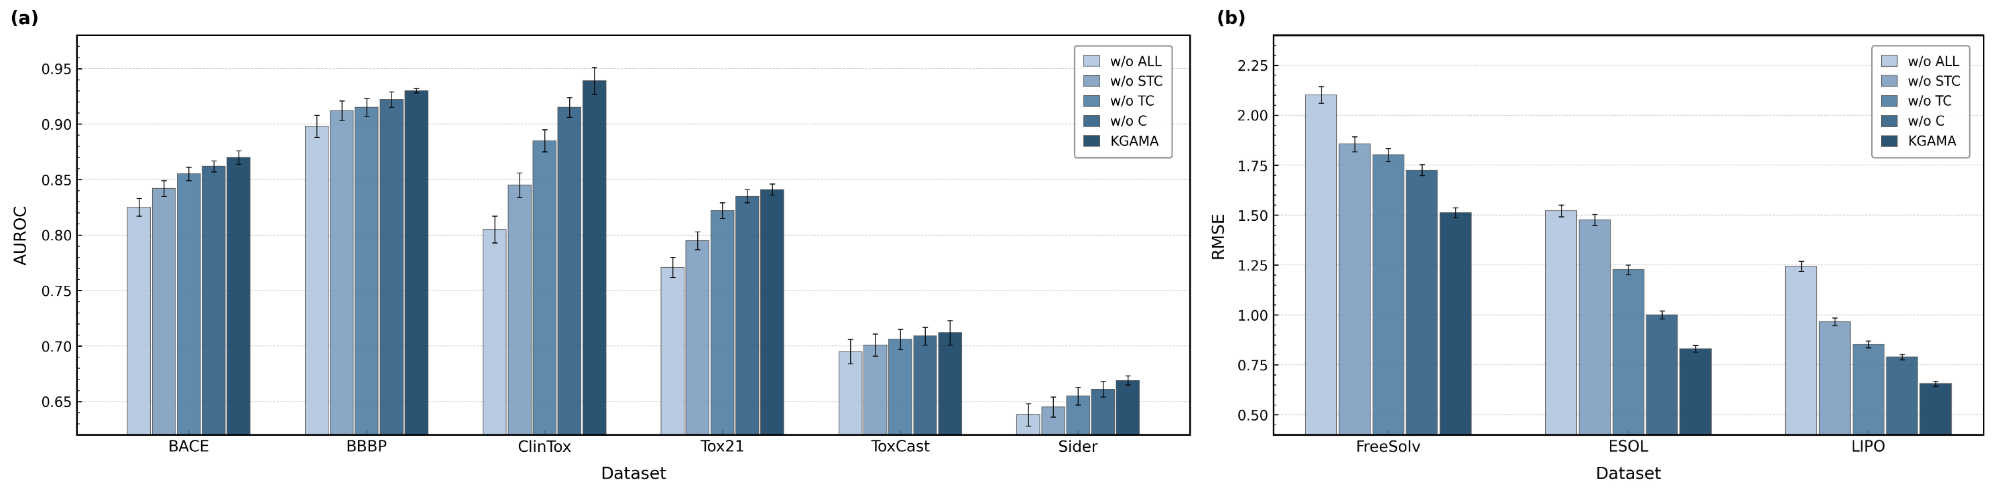
\includegraphics[width=\textwidth]{figures/fig6_class_reg_ablation.png}
    \caption{Ablation results of KGAMA on the MoleculeNet benchmark tasks. (a) Classification performance measured by AUROC. (b) Regression performance measured by RMSE.}
    \label{fig:combined-ablation}
\end{figure*}

\subsection{Visualization analysis}
To better interpret modality usage across tasks, we analysed the learned attention weights assigned to graph, sequence, fingerprint and text branches. The resulting weighting patterns were strongly task dependent and broadly consistent with chemical intuition, as shown in Figure~\ref{fig:modality-weights}.

For physicochemical regression tasks such as ESOL and FreeSolv, the graph modality dominated, indicating that the structural topology captured by Graphormer provides the most informative signal for solubility- and solvation-related properties. By contrast, the fingerprint branch received the highest contribution on Lipophilicity, consistent with the dependence of lipophilicity on the occurrence of characteristic hydrophobic and hydrophilic functional groups.

For biologically complex tasks such as SIDER, ClinTox and Tox21, the text modality received markedly higher attention weights. This pattern suggests that the rewritten and descriptor-enriched text branch captures pharmacological semantics that are difficult to infer from structure alone. The relative stability of the SMILES branch across tasks indicates that sequence features provide a robust complementary view without dominating multimodal integration.

\begin{figure*}[t]
    \centering
    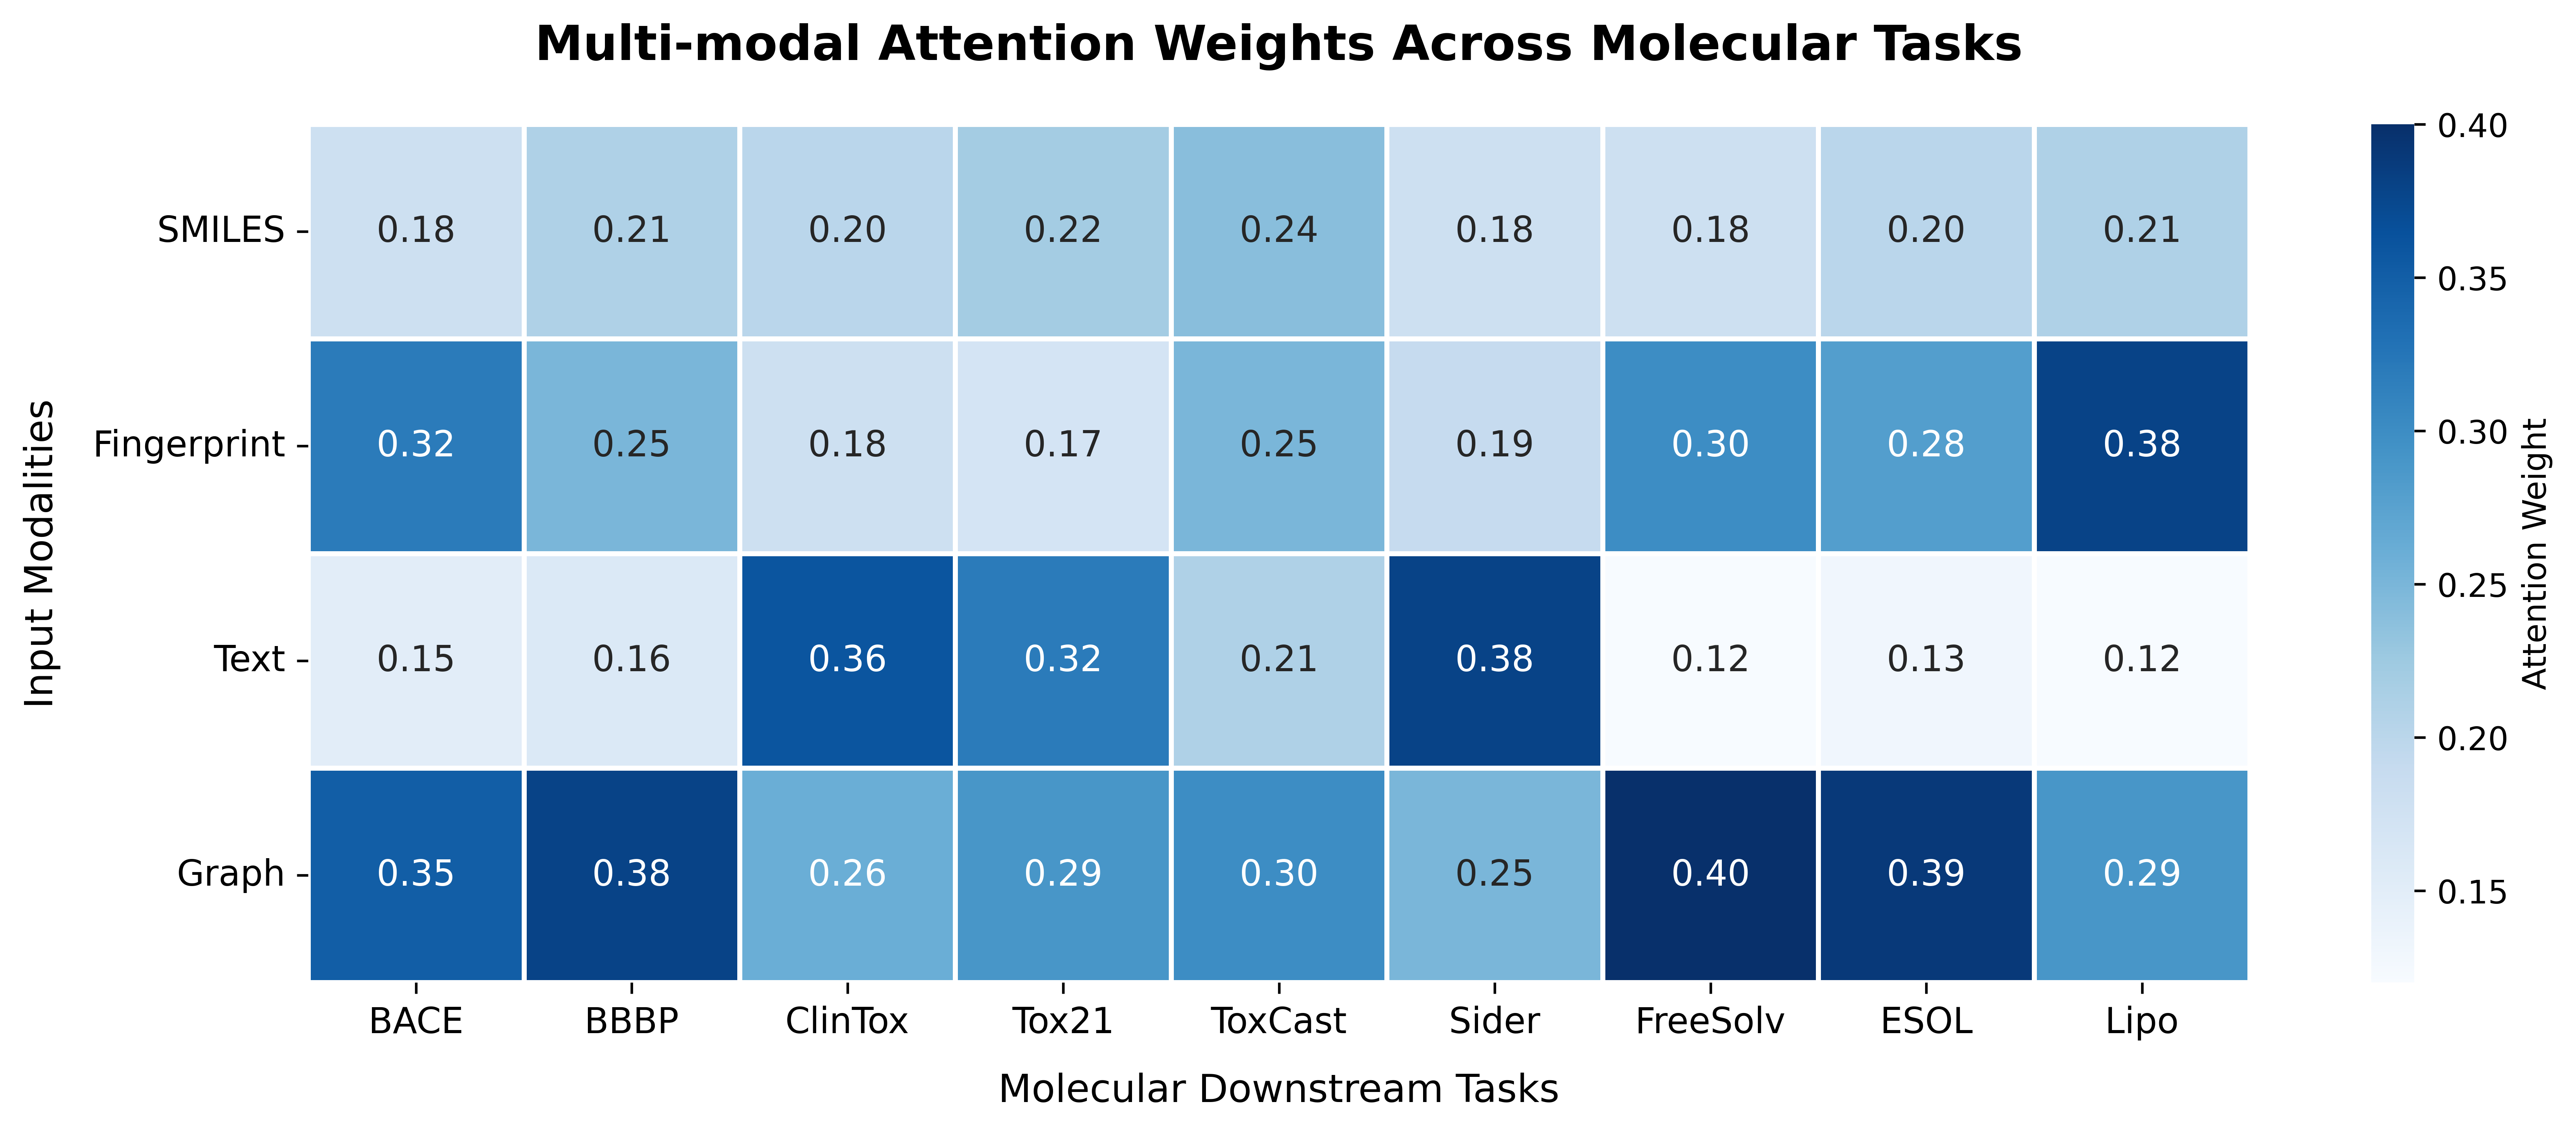
\includegraphics[width=0.82\textwidth]{figures/fig4_modality_weights.png}
    \caption{Learned modality attention weights across downstream molecular property prediction tasks. Darker colors indicate higher contribution from the corresponding modality.}
    \label{fig:modality-weights}
\end{figure*}

\subsection{Parameter sensitivity}
We further investigated the sensitivity of KGAMA to the temperature parameter in the NT-Xent loss on representative datasets. The performance curve followed a clear inverted-U pattern as the temperature increased from 0.05 to 1.0, as shown in Figure~\ref{fig:temperature-sensitivity}. Very small temperature values overemphasized hard negatives and destabilized optimization, whereas large values reduced discrimination among non-matching samples. The best results were obtained around 0.1, which was therefore used in all subsequent experiments.

\begin{figure*}[t]
    \centering
    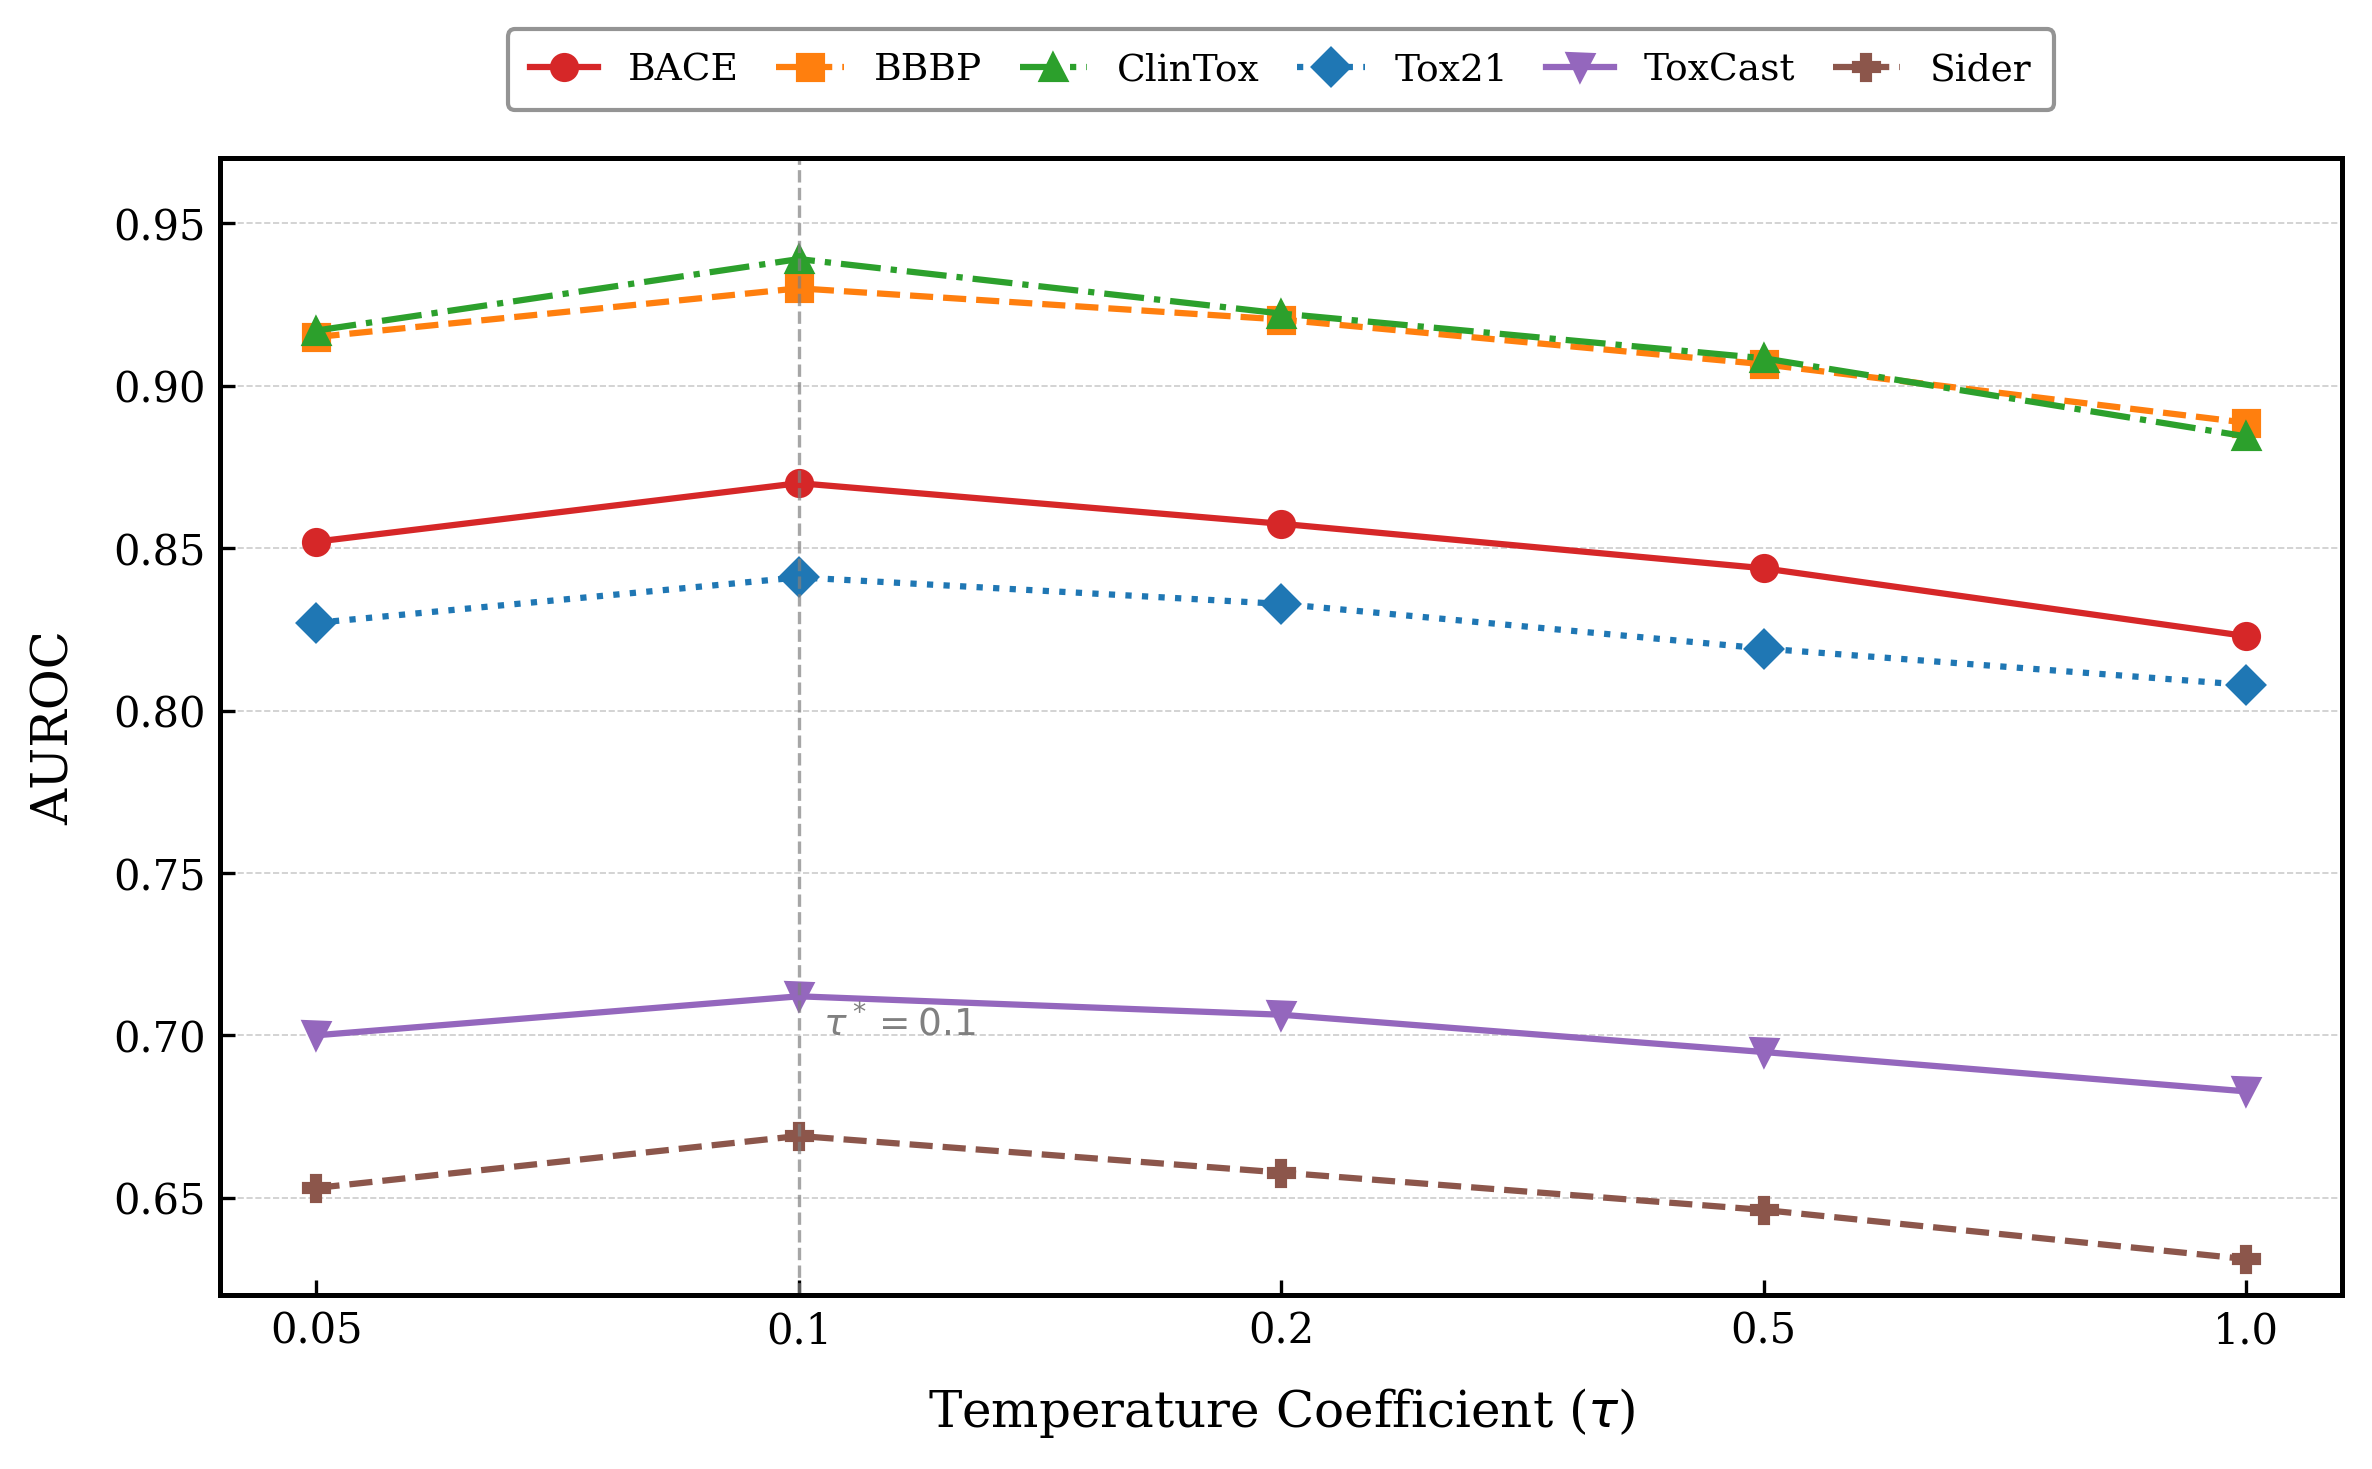
\includegraphics[width=0.82\textwidth]{figures/fig5_temperature_sensitivity.png}
    \caption{Sensitivity of KGAMA to the temperature coefficient $\tau$ in the NT-Xent loss across representative classification benchmarks. The best overall performance is obtained around $\tau=0.1$.}
    \label{fig:temperature-sensitivity}
\end{figure*}

\section{Discussion}
The results suggest that two design choices are particularly important for robust multimodal molecular learning. The first is the explicit improvement of textual quality before representation learning. Raw public-domain molecular text is often weakly aligned with downstream prediction objectives, whereas the rewritten text in KGAMA is shorter, denser and more chemically constrained through the inclusion of RDKit-derived descriptors. This appears to be especially useful for tasks involving toxicity and side effects, where expert-style semantic information can provide cues beyond purely structural representations.

The second is the graph-centered alignment strategy. Instead of imposing full pairwise alignment across all modalities, KGAMA uses the molecular graph as the central semantic anchor and aligns the auxiliary views against this anchor. This reduces unnecessary matching among noisy auxiliary modalities and provides a more stable optimization target. The uncertainty-aware weighting mechanism further improves robustness by allowing the model to modulate the contribution of each contrastive objective during training.

Although KGAMA shows strong overall results, several limitations remain. First, the present study focuses on 2D graph structure and does not explicitly incorporate 3D conformational information, which could be important for some biochemical endpoints. Second, the rewritten text depends on the quality of upstream retrieval and language model generation. Third, while the current benchmarks cover diverse tasks, broader external validation would be valuable for assessing generalization in realistic medicinal chemistry settings.

Future work may therefore extend the framework in three directions: incorporating geometric molecular representations, strengthening automatic quality control for rewritten text, and evaluating the model on larger and more heterogeneous benchmark collections. Despite these limitations, the present results indicate that multimodal molecular prediction benefits substantially from chemically grounded semantic alignment and task-adaptive knowledge enhancement.

\section{Conclusion}
We presented KGAMA, a knowledge-enhanced graph-anchor multimodal alignment framework for molecular property prediction. KGAMA integrates molecular graphs, SMILES, fingerprints and rewritten scientific text within a pretraining--finetuning pipeline, combines graph-centered contrastive alignment with uncertainty-aware adaptive weighting, and uses cross-attention for downstream multimodal fusion. Across 9 MoleculeNet benchmarks, the method delivered strong and consistent performance on both classification and regression tasks. These findings indicate that knowledge-enhanced text construction and graph-centered multimodal alignment are effective strategies for improving molecular representation learning and downstream property prediction.

\section{Conflicts of interest}
The authors declare that they have no competing interests.

\section{Funding}
Funding information will be added here.

\section{Data availability}
The benchmark datasets analysed in this study are available from the corresponding public sources, including MoleculeNet and PubChem. Processed data and code will be released upon acceptance.

\section{Author contributions statement}
S.F. conceived the study, designed the methodology, implemented the model, performed the experiments, analysed the results and drafted the manuscript.

\section{Acknowledgments}
The authors thank all contributors to the public molecular databases and benchmark resources used in this study.

\begin{thebibliography}{99}

\bibitem{placeholder1}
References will be added and formatted in the next revision.

\end{thebibliography}

\end{document}
